%
% robertson.tex -- Robertson Walker Metrik
%
% (c) 2017 Prof Dr Andreas Müller, Hochschule Rapperswil
%
\chapter{Kosmologie%
\label{skript:chapter:kosmologie}}
\lhead{Kosmologie}
\rhead{}
Die Einstein-Gleichungen ermöglichen erstmals, die Entwicklung
des ganzen Universums zu modellieren.
Dazu sind allerdings die Kenntnis der grossräumigen
Masseverteilung notwendig.
Es stellt sich heraus, dass diese im grossen isotrop und homogen ist.
Dies bedeutet, dass auch die Krümmung im Universum homogen und isotrop
ist.
Die Robertson-Walker-Metrik erfüllt diese Voraussetzung.

\section{Expansion des Universums}
\rhead{Expansion}
Zu Beginn des 20.~Jahrhunderts hatte man noch keine klare Vorstellung
über die Grösse des Universums.
Allgemein wurde angenommen, dass unsere Milchstrasse im wesentlichen das
ganze Universum ist.
Die seit längerer Zeit bekannten Nebel wurden als Teil der Milchstrasse
angesehen.
Auch wurde das Universum im wesentlichen als unveränderlich angesehen.

In den frühen zwanziger Jahren des 20.~Jahrhunderts gelang es dann
Edwin Hubble, die Entfernung von Andromeda und anderen heute als
Galaxien bekannten Nebeln zu bestimmen.
Er verwendete dafür sogenannte Cepheiden-Veränderliche.
Zwischen der absoluten Helligkeit dieser veränderlichen
Sterne und der Periode der Helligkeitsschwankungen besteht
eine einfache Beziehung.
Hubble fand Cepheiden-Veränderliche in Aufnahmen der Andromeda-Galaxie
und war damit in der Lage, deren absolute Helligkeit zu bestimmen.
Aus der beobachteten Helligkeit konnte er die Entfernung ableiten.
Es zeigte sich, dass diese Galaxien weit ausserhalb unserer Milchstrasse
befinden.

Hubble und sein Assistent Milton Humason massen mit dem neuen
2.5m-Hooker-Teleskop neben der Entfernung auch die Spektren und
damit die Rotverschiebung von 46 Galaxien.
Es zeigte sich, dass sich weiter entfernte Galaxien schneller 
entfernen.
Sie schlossen daraus, dass das Universum expandieren muss, sie konnten
sogar die Geschwindigkeit bestimmen, mit der dies geschieht.

Der belgische Physiker
Georges Lemaître hatte auf der Basis von Einsteins allgemeiner
Relativitätstheorie die Expansion des Universums bereits vor
Hubbles Entdeckung vorhergesagt.
Doch erst mit die Messungen von Hubble und Humason haben bewiesen,
dass Einsteins Theorie die Entwicklung des Universums korrekt
vorhersagen kann.

\subsection{Der Skalenfaktor}
\begin{figure}
\centering
\includegraphics[width=\hsize]{chapters/tikz/expansion1.pdf}
\caption{Expansion des Universums um einen Beobachter im ``Zentrum''
\label{skript:figure:expansion1}}
\end{figure}
\begin{figure}
\centering
\includegraphics[width=\hsize]{chapters/tikz/expansion2.pdf}
\caption{Expansion des Universums. Da sich das Univerum überall
mit dem gleichen Skalenfaktor ausdehnt, erscheinen sich für jeden
Beobachter die Galaxien mit der gleichen Geschwindigkeit zu entfernen.
Die Fluchgeschwindigkeit ist kein Hinweis darauf, dass im Universum
einen bevorzugten Punkt gäbe (Homogenität).
\label{skript:figure:expansion2}}
\end{figure}
Hubbles Beobachtungen haben gezeigt, dass sich das Universum ausdehnt.
Zwei nahe Punkte befinden sich zur Zeit $t_0$ in einem Abstand $d_0$,
und sollen in einem geeigneten Koordinatensystem in Ruhe sein.
Zu einer späteren Zeit wird die Distanz sich vergrössert haben.
Da das Universum isotrop und homogen ist, muss die Distanz in jeder
beliebigen Richtung um den gleichen Faktor gewachsen sein.
Die Ausdehnung des Universums ist also eine Ähnlichkeitstransformation.
Sie kann durch eine einzige, von der Zeit abhängige Zahl,
den {\em Skalenfaktor} $a(t)$ beschrieben werden.
\index{Skalenfaktor}
Wir geben der Funktion $a(t)$ willkürlich den Wert $1$ für die heutige
Zeit.

Die Tatsache, dass ein Beobachter alle Galaxien sich entfernen
sieht bedeutet nicht, dass das Universum ein Zentrum.
Auch für jeden anderen Beobachter werden die Distanzen zu den
Galaxien grösser und zwar um den gleichen Faktor
(Abbildungen~\ref{skript:figure:expansion1} und
\ref{skript:figure:expansion2}).

\subsection{Die Hubble-Konstante und das Alter des Universums}
Nehmen wir an, dass das Universum sich mit konstanter Geschwindigkeit
ausdehnt, dass also 
\[
H(t)=H_0=\frac{\dot a(t)}{a(t)}
\]
gilt.
Dies ist eine Differentialgleichung für $a(t)$, die wir sofort
lösen können:
\[
a(t) = H_0a(t)
\qquad \Rightarrow\qquad
a(t)=H_0 e^{t-t_0}
\]
Wir erhalten daher einen exponentiell anwachsenden Skalenfaktor,
wofür es keinen experimentellen Hinweis gibt, und der auch physikalisch
unsinnig scheint.
$H(t)$ kann also keine Konstante sein.

Nehmen wir aber an, dass $\dot a(t)$ konstant ist, dann ist $a(t)$
eine lineare Funktion der Zeit mit Steigung  $H_0$ zur Zeit $t=t_0$,
also
\[
a(t)=H_0(t-t_0) + 1.
\]
Daraus können wir den Zeitpunkt berechnen, zu dem der Skalenfaktor
$a(t)=0$ war, es muss
\[
t-t_0 = -\frac1{H_0}
\]
gelten.
Man nennt $1/H_0$ die {\em Hubble-Zeit}.
\index{Hubble-Zeit}
Der beste bekannte Wert für $H_0$ wurde mit der Planck-Mission als
\index{Planck-Mission}
\begin{equation}
H_0
=
(67.74 \pm 0.46)\frac{\text{km}}{\text{s}\cdot\text{Mpc}}
=
(2.1951\pm 0.0149)
10^{-18}\frac{1}{\text{s}}
\label{skript:robertson:hubble0}
\end{equation}
bestimmt.
Die zugehörige Hubble-Zeit ist
\begin{equation}
\frac{1}{H_0} = 14.4\text{Gyr}.
\label{skript:robertson:hubblezeit}
\end{equation}
Wenn wir annehmen, dass die im Universum enthaltene Masse die Ausdehnung
verlangsamt, muss die Hubble-Zeit eine obere Schranke für das Alter
des Universums sein.

\section{Masseverteilung im Universum}
\rhead{Masseverteilung im Universum}
Lange Zeit galt die Erde als das Zentrum des Universums.
Nikolaus Kopernikus hat mit dem heliozentrischen Modell der Erde
diese privilegierte Stellung genommen.
Wilhelm Herschel war der erste Astronom, der sich darüber Gedanken
gemacht hat, wo innerhalb unserer Milchstrasse unser Sonnensystem
einzuordnen wäre.
Heute wissen wir, dass die Erde eher am Rande der Milchstrasse liegt.
Doch auch die Milchstrasse ist nichts besonderes, sie ist eine eher
unterdurchschnittliche Galaxie in einem durchschnittlichen
Galaxienhaufen.
Man kann diese Beobachtungen zusammenfassen im sogenannten
{\em kosmologischen Prinzip}, welches besagt, dass an unserem
Standort im Universum nichts speziell ist.

\subsection{Isotropie}
Isotropie bedeutet, dass es im Universum keine bevorzugte Richtung
gibt.
Auf kurze Distanzen stimmt dies ganz offensichtlich nicht.
In einer Kugel von wenigen Metern Durchmesser um den Beobachter
gibt es eine objektiv bevorzugte Richtung, die Richtung des Schwerfeldes
der Erde zum Erdmittelpunkt,
Aber auch in einer Kugel von etwa einer Milliarde Kilometer um
den Beobachter gibt es eine bevorzugte Richtung, nämlich die
Richtung zum hellsten und massivsten Stern, der Sonne.
Selbst in einer Kugel von etwa 3~Mpc\footnote{Mpc = 1 Million parsec,
ein parsec entspricht $30.857\cdot 10^{16}\text{m} = 3.26\text{Lichtjahre}$.}
kann man eine bevorzugte Richtung finden, nämlich die Richtung zur grössten
und hellsten Galaxie des lokalen Haufens, der Andromeda-Galaxie M31.
Erst in einer Kugel mit einem Radius von etwa 100Mpc gibt es keine
bevorzugte Richtung mehr. 

\subsection{Homogenität}
Homogenität bedeutet, dass es keinen bevorzugten Standort im Universum gibt.
Auf kurze Distanzen gilt dies ganz offensichtlich nicht.
In einer Kugel von einigen tausend Kilometern um den Beobachter ist
die Erde als massivstes Objekt ein bevorzugter Standort.
In einer Kugel von einer Milliarde Kilometer um den Beobachter ist
die Sonne als massivstes hellstes Objekt bevorzugt.
In einer Kugel von 100000 Lichtjahren um den Beobachter ist das Zentrum
der Milchstrasse mit dem dortigen supermassiven schwarzen Loch ein
bevorzugter Ort.
In einer Kugel von etwa 3~Mpc ist der Schwerpunkt des Lokalen Galaxienhaufens
ein bevorzugter Ort.
Bei grösseren Radien findet man zwar noch Cluster von Galaxien und
Supercluster, also Cluster von Galaxienclustern, aber jenseits von
etwa 100 Mpc scheint es keine noch grösseren Strukturen mehr zu geben.
In diesen Grössenordnungen kann man daher das Universum als homogen
bezeichnen.


\subsection{Energie-Impuls-Tensor}

\section{Robertson-Walker-Metrik}
\rhead{Robertson-Walker-Metrik}
Das Universum ist auf grosse Distanzen homogen und isotrop.
Die Einstein-Gleichungen müssen daher auch eine Metrik als
Lösung zulassen, die homogen und isotrop ist.
In diesem Abschnitt wollen wir untersuchen, wie die Metrik eines
solchen Raums beschaffen sein muss.

\subsection{Zeit}
Wenn kein Standort im Universum bevorzugt ist, dann muss es
eine universelle Zeitkoordinaten $t$ geben, die Metrik muss
sich schreiben lassen in der Form
\[
ds^2
=
-c^2\,dt^2
+
g_{ij}\,dx^i\,dx^j
\]
wobei wie früher lateinische Indizes andeuten sollen, dass die
Summation nur über die Raumkoordinaten zu erstrecken ist.
Wäre dies nicht möglich, dann müsste der Koeffizient von $dt^2$
in einem Raumpunkt von $-c^2$ abweichen.
Dieser Punkt hätte dann aber andere Eigenschaften als alle anderen
Punkte im Universum, was das kosmologische Prinzip verletzt.

\subsection{Isotrop und homogen gekrümmte Räume}
Wir suchen jetzt eine Metrik des dreidimensionalen Raumes, welche
isotrop und homogen ist.
Der euklidische Raum mit der Metrik
\[
g_{ij}dx^i\,dx^j
=
dx^2 + dy^2 + dz^2
\]
ist sicher homogen und isotrop. 
Er ist aber auch flach, und daher zu wenig allgemein als mögliches
Modell für das Universum.
Die euklidische Metrik kann auch in Kugelkoordinaten als
\begin{equation}
ds^2
=
dr^2
+ 
r^2\,d\vartheta^2
+
r^2\sin^2\vartheta\,d\varphi^2
\label{skript:rwmetrik:kugelkoordinaten}
\end{equation}
geschrieben werden.
Die letzten zwei Terme~\eqref{skript:rwmetrik:kugelkoordinaten}
zeigen scheinbar eine bevorzugte Richtung, nämlich die Richtung
des Nord- und Südpols.
Dies ist jedoch nur ein Artefakt des Koordinatensystems, die 
Längenmessung ist davon nicht betroffen.
Wir können dies dadurch ausdrücken, dass wir die zwei Terme
zusammenfasssen als
\begin{equation}
d\Omega^2 = d\vartheta^2 + \sin^2\vartheta\,d\varphi^2.
\end{equation}
Damit kann die Metrik abgekürzt als
\begin{equation}
ds^2 = dr^2 + r^2\,d\Omega^2
\end{equation}
geschrieben werden.
Der Terme $r^2\,d\Omega^2$ beschreibt die Längenmessung auf der
``Kugel'' bei der Koordinaten $r$ um den Nullpunkt des
Koordinatensystems.

Da das Universum isotrop ist, darf keine Richtung ausgezeichnet sein.
Insbesondere muss eine von der euklidischen Metrik abweichende
Metrik immer noch unverändert den Teil $d\Omega^2$ enthalten.
Es ist aber zulässig, dass die Längenmessung auf der Kugel sich
gegenüber der Längenmessung in radialer Richtung verändert hat.
Man beobachtet dies zum Beispiel auch in der Umgebung eines Punktes
auf einer Kugeloberfläche: je weiter man sich von diesem Punkt entfernt,
desto kleiner wird der Umfang eines Kreises um den Punkt im Vergleich
zum Radius. 
Ist der Radius des Kreises $\frac{\pi}2R$, wobei $R_c$ der Kugelradius ist,
dann ist der Umfang $U$ des Kreises
\[
U=2\pi R_c \ne 2\pi \cdot r = 2\pi\frac{\pi}2R_c=\pi^2 R_c.
\]
Wir suchen daher eine Metrik in der Form
\[
ds^2 
=
dr^2 + S(r)^2 \,d\Omega^2,
\]
wobei $S(r)$ für einen euklischen Raum $S(r)=r$ ist.
Ein Kreis mit Radius $r$ hat in dieser Metrik den Umfang
\[
U=\int_{\textrm{Kreis}} S(r)\,d\Omega = 2\pi S(r).
\]
Auch wenn für einen gekrümmten Raum $S(r)$ nicht mehr gleich $r$ ist,
muss weiterhin $S(0)=0$ gelten, wenn der Radius verschwindet, dann
hat der zugehörige Kreis auch verschwindenden Umfang.
Für kleine Radien $r$ muss ausserdem die Geometrie kaum von der
euklidischen unterscheidbar sein, es muss also $S(r)\simeq r$ gelten,
oder $S'(r)=1$,
Die Funktion $S(r)$ muss daher die Anfangsbedingungen
\begin{equation}
\begin{aligned}
S(0)&=0&&\qquad&S'(0)&=1
\end{aligned}
\label{skript:rwmetrik:Safangsbedingungen}
\end{equation}
erfüllen.

\subsubsection{Krümmung}
Die Funktion $S(r)$ ist nun also so zu bestimmen, dass der Raum auch
homogen ist.
Um sie zu bestimmen verwenden wir wieder die Analogie zur Oberfläche
einer zweidimensionalen Kugel mit Radius $R_c$.
Zu einem Kreis mit Radius $r$ im den Nordpol gehört der Winkel
$\vartheta$ mit $\vartheta = r/R$.
Der Umfang dieses Kreises ist dann
\[
2\pi R_c\sin\vartheta
=
2\pi S(r)
\]
der
\[
S(r) = R_c\sin\vartheta=R\sin\frac{r}{R_c}.
\]
In der zu dieser Funktion $S(r)$ gehörigen Metrik hat ein Kreis mit 
Radius $r=\pi R$ Umfang $0$, dies entspricht dem Antipodenpunkt des
Nullpunktes.

Bis jetzt haben wir uns von der Anschauung leiten lassen, ohne den
Begriff der Krümmung zu verwenden.
Um die allgemeine Lösung für $S(r)$ zu finden, können wir
aber auch verlangen, dass die Metrik
\[
dr^2 + S(r)^2\,d\Omega^2
\]
überall die gleiche Krümmung hat.
Wir berechnen daher für diese Metrik den Ricci-Krümmungsskalar.
Diese Rechnung ist ziemlich aufwendig, kann aber mit Maxima
mit Hilfe des Programms von Seite~\pageref{skript:maxima:curvature}
ohne
Schwierigkeit ausgeführt werden.
\lstinputlisting[style=Maxima]{chapters/robertson3.maxima}
Man erhält 
\verbatiminput{chapters/robertson3.txt}
oder in konventioneller Notation
\[
R=
-\frac{2S''(r)}{S(r)}
\]
und damit die Bedingung
\begin{equation}
S''(r)=-2k S(r)
\label{skript:rwmetrik:Sdgl}
\end{equation}
für $S(r)$ und eine geeignete Konstante $k$.
Gleichung \eqref{skript:rwmetrik:Sdgl} ist eine gewöhnliche
Differentialgleichung zweiter Ordnung.

\subsubsection{Lösung der Differentialgleichung für $S_\kappa(r)$}
Die Differentialgleichung~\eqref{skript:rwmetrik:Sdgl}
muss mit den Anfangsbedingungen~\eqref{skript:rwmetrik:Safangsbedingungen}
gelöst werden.
Falls $k$ positiv ist, folgt
\begin{equation}
S(r)=\frac1{\sqrt{2k}}\sin(\sqrt{2k}\,r) = R_c\sin\frac{r}{R_c}
\qquad\text{mit}\qquad
R_c=\frac1{\sqrt{2k}}.
\label{skript:rwmetrik:sinloesung}
\end{equation}
Dies ist der Fall, den wir bereits durch die geometrische Analogie mit
der zweidimensionalen Sphäre gefunden haben.

Die Gleichung~\eqref{skript:rwmetrik:Sdgl} hat aber noch eine weitere 
Lösungen.
Für negatives $k$ folgt wieder unter Verwendung der
Anfangsbedingung~\eqref{skript:rwmetrik:Safangsbedingungen}
\begin{equation}
S(r)=\frac{1}{\sqrt{-2k}}\sinh(\sqrt{-2k}\, r)
=
R_c\sinh\frac{r}{R_c}
\qquad\text{mit}\qquad
R_c=\frac1{\sqrt{-2k}}.
\label{skript:rwmetrik:sinhloesung}
\end{equation}
Diese Lösung gehört zu einem Raum mit negativer Krümmung.
Sogar den euklidische Fall können wir für $k=0$ wiedergewinnen, es folgt
dann $S(r)=r$.

\begin{figure}
\centering
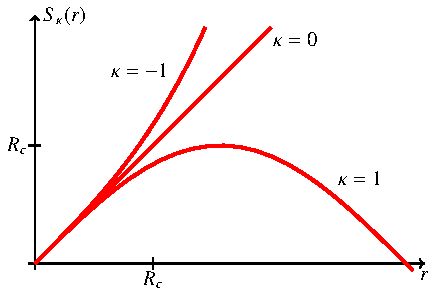
\includegraphics{chapters/tikz/robertson.pdf}
\caption{Darstellung der Funktionen $S_\kappa(r)$ für $R_c=1$ und
verschiedene Werte von $\kappa$
\label{skript:Skappa:graph}}
\end{figure}

Offenbar spielt für die Lösung  nur das Vorzeichen von $k$ und die
Grösse $R_c$ ein Rolle.
Wir können $S(r)$ daher auch etwas einheitlicher als
\begin{equation}
S_\kappa(r) = \begin{cases}
R_c\sin  \displaystyle\frac{\mathstrut r}{R_c} &\qquad \kappa= 1\\
r                                              &\qquad \kappa= 0\\
R_c\sinh \displaystyle\frac{\mathstrut r}{R_c} &\qquad \kappa=-1
\end{cases}
\label{skript:rwmetrik:Skappa}
\end{equation}
schreiben.
In Abbildung~\ref{skript:Skappa:graph} sind die Funktionen $S_\kappa(r)$
für $R_c=1$ und für alle drei Werte von $\kappa$ dargestellt.
Ebenfalls erkennbar ist, dass für kleine Werte von $r$ gilt
$S_\kappa(r)\simeq r$.

\subsubsection{Ableitungen von $S_\kappa(r)$}
Für spätere Verwendung berechnen wir die erste und zweite Ableitung 
von $S_\kappa(r)$.
Die erste Ableitung ist
\begin{align*}
S'_\kappa(r)
&=
\begin{cases}
\cos \displaystyle\frac{\mathstrut r}{R_c}&\qquad \kappa= 1\\
1                                         &\qquad \kappa= 0\\
\cosh\displaystyle\frac{\mathstrut r}{R_c}&\qquad \kappa=-1
\end{cases}
\end{align*}
In Hinblick auf spätere Verwendung in der Friedmann-Gleichung drücken wir
die rechte Seite durch $S_\kappa(r)$ aus. 
\begin{equation}
S'_\kappa(r)^2
=
\left\{
\begin{aligned}
&\cos^2\displaystyle\frac{\mathstrut r}{R_c}
=
1-\sin^2\displaystyle\frac{\mathstrut r}{R_c}
=
1-\kappa \frac{S_\kappa(r)^2}{R_c^2}&&\qquad\kappa=1\\
&1&&\qquad\kappa=0\\
&\cosh^2\displaystyle\frac{\mathstrut r}{R_c}
=
1+\sinh^2\displaystyle\frac{\mathstrut r}{R_c}
=
1-\kappa \frac{S_\kappa(r)^2}{R_c^2}&&\qquad\kappa=-1
\end{aligned}
\right.
\end{equation}
Unabhängig vom Wert von $\kappa$ und $R_c$ gilt also immer
\begin{equation}
S'_\kappa(r)^2 = 1-\kappa \frac{S_\kappa(r)^2}{R_c^2}.
\label{skript:robertson:ersteableitung}
\end{equation}
Für die zweite Ableitung finden wir
\begin{align*}
S''_\kappa(r)
&=
\begin{cases}
\displaystyle-\frac{1}{R_c}\sin \frac{\mathstrut r}{R_c}&\qquad \kappa= 1\\
0                                                       &\qquad \kappa= 0\\
\displaystyle \frac{1}{R_c}\sinh\frac{\mathstrut r}{R_c}&\qquad \kappa=-1
\end{cases}
\end{align*}
Auch dieses Resultat können wir einheitlich als
\begin{equation}
S''_\kappa(R)
=
-\kappa\displaystyle \frac{S_\kappa(r)}{R_c^2}
\label{skript:robertson:zweiteableitung}
\end{equation}
schreiben.

Eine homogene und isotrope Metrik eines dreidimensionalen Raumes
hat daher die Form
\begin{equation}
ds^2=dr^2 + S_{\kappa}(r)d\Omega^2.
\label{skript:rwmetrik:metrikS}
\end{equation}
Diese Metrik beschreibt einen Raum mit konstanter Krümmung.
Der Parameter $\kappa$ kann nur die Werte $\pm 1$ und $0$ annehmen.
Für $\kappa=1$ ist die Krümmung des Raumes positiv, für $\kappa=-1$ ist
sie negativ, für $\kappa=0$ liegt ein euklidischer Raum vor.
Der Krümmungsradius ist in den Fällen $\kappa=\pm1$ jeweils $R_c$.

\subsubsection{Der Grenzfall $R_c\to\infty$}
Schreibt man $K_c = 1/R_c$ für die Krümmung, dann kann man $S_0(r)$
auch als Grenzfall von $S_{\pm 1}(r)$ für $K_c\to 0$ erhalten.
Es gilt  nämlich
\begin{equation}
\lim_{R_c\to\infty} S_\kappa(r)
=
\lim_{K_c\to 0} S_\kappa(r)
=\begin{cases}
\displaystyle
\lim_{K_c\to 0}\frac{\displaystyle \sin(K_cr)}{\displaystyle K_c}
=
\lim_{K_c\to 0}\frac{\displaystyle r\cos(K_cr)}{\displaystyle 1} = r = S_0(r)
&\qquad\kappa=1
\\
\\
\displaystyle
\lim_{K_c\to 0}\frac{\displaystyle \sinh(K_cr)}{\displaystyle K_c}
=
\lim_{K_c\to 0}\frac{\displaystyle r\cosh(K_cr)}{\displaystyle 1} = r = S_0(r)
&\qquad\kappa=-1
\end{cases}
\end{equation}
nach der Regel von de l'Hospital.
Die Funktion $S_0(r)$ ist daher der Grenzfall der Funktionen
$S_\kappa(r)$ für unendlich grossen Krümmungsradius $R_c$.

\subsection{Robertson-Walker-Metrik}
Da wir jetzt die Zeitabhängigkeit wie auch die Ortsabhängigkeit der
Metrik eines isotropen und homogen gekrümmten Raumes kennen, können
wir die allgemeinste Form der vierdimensionalen Metrik eines solchen
Raumes gefunden.

\begin{satz}
Ein homogenes, isotropes Universum hat eine Metrik der Form
\[
ds^2
=
-c^2 dt^2 + a(t)^2\bigl(
dr^2 + S_\kappa(r)^2(d\vartheta^2 + \sin^2\vartheta\, d\varphi^2)
\bigr)
\]
mit $\kappa\in\{0,\pm1\}$ und 
$S_\kappa(r)$ ist eine der Funktionen
\[
S_\kappa(r)
=
\begin{cases}
R_c\sin \displaystyle\frac{\mathstrut r}{R_c}&\qquad \kappa= 1\\
r&\qquad \kappa=0\\
R_c\sinh\displaystyle\frac{\mathstrut r}{R_c}&\qquad \kappa=-1
\end{cases}
\]
\end{satz}

Wir bestimmen die Geodätengleichungen in der Robertson-Walker Metrik.
Die allgemeine Geodätengleichung hat die Form
\[
\frac{d^2x^\mu}{ds^2} = -\Gamma^\mu_{\alpha\beta} \dot x^\alpha \dot x^\beta.
\]
Man muss also als erstes die Christoffelsymbole bestimmen.  
Diese sind auch deshalb interessant, weil $\Gamma^0_{kk}$ in erster
Näherung die Gravitationskräfte beschreibt.

Für jeden Index $\mu$ bilden die $\Gamma^\mu_{\alpha\beta}$
eine symmetrische Matrix.
Für $\mu=0$ zum Beispiel finden wir
\begin{align*}
\Gamma^0_{\alpha\beta}
&=
\begin{pmatrix}
%(%i5) 		        ratsimp(Christoffel2(1, 1, 1))
%(%o5) 				       0
%(%i6) 		        ratsimp(Christoffel2(1, 1, 2))
%(%o6) 				       0
%(%i7) 		        ratsimp(Christoffel2(1, 1, 3))
%(%o7) 				       0
%(%i8) 		        ratsimp(Christoffel2(1, 1, 4))
%(%o8) 				       0
0&0&0&0\\
%(%i9) 		        ratsimp(Christoffel2(1, 2, 2))
%				     d
%			       a(t) (-- (a(t)))
%				     dt
%(%o9) 			       ----------------
%				       2
%				      c
%(%i10) 		        ratsimp(Christoffel2(1, 2, 3))
%(%o10) 				       0
%(%i11) 		        ratsimp(Christoffel2(1, 2, 4))
%(%o11) 				       0
0&\frac1{c^2} a(t)\dot a(t)& 0 & 0 \\
%(%i12) 		        ratsimp(Christoffel2(1, 3, 3))
%			     2	        d
%			    S (r) a(t) (-- (a(t)))
%					dt
%(%o12) 			    ----------------------
%				       2
%				      c
%(%i13) 		        ratsimp(Christoffel2(1, 3, 4))
%(%o13) 				       0
0 & 0 & \frac1{c^2}a(t)\dot a(t)S_\kappa(r)^2 & 0 \\
%(%i14) 		        ratsimp(Christoffel2(1, 4, 4))
%		       2	  d	        2
%		      S (r) a(t) (-- (a(t))) sin (theta)
%				  dt
%(%o14) 		      ----------------------------------
%				       2
%				      c
0 & 0 & 0 & \frac1{c^2} a(t)\dot a(t)S_\kappa(r)^2 \sin^2\vartheta
\end{pmatrix}
\\
&=
\frac1{c^2}
\frac{\dot a(t)}{a(t)}
\begin{pmatrix}
0&     0&                  0&                                 0\\
0&a(t)^2&                  0&                                 0\\
0&     0&a(t)^2S_\kappa(r)^2&                                 0\\
0&     0&                  0&a(t)^2S_\kappa(r)^2\sin^2\vartheta
\end{pmatrix}
\end{align*}
Die Matrix in der letzten Zeile stimmt bis auf die $00$-Komponente
mit der Metrik überein.
Der Faktor $\dot a(t)/a(t)$ beschreibt die Ausdehungsgeschwindigkeit
des Universums.

\subsection{Die Ausdehnung des Universums}
Aus Metrik eines homogenen und isotropen Raumes gemäss
\eqref{skript:rwmetrik:metrikS}
können wir jetzt die allgemeine Metrik einer homogenen und
isotropen Raumzeit konstruieren.
Die Metrik
\begin{equation}
ds^2
=
-c^2\,dt^2 
+
a(t)^2\bigl( dr^2 + S_\kappa(r) \,d\Omega^2\bigr)
\label{skript:rwmetrik:rwmetrik}
\end{equation}
heisst die Robertson-Walker-Metrik.
Wir können sie verwenden, um die Entwicklung des Universums zu
modellieren.

\section{Wie ist das Universum gekrümmt?}
\begin{figure}
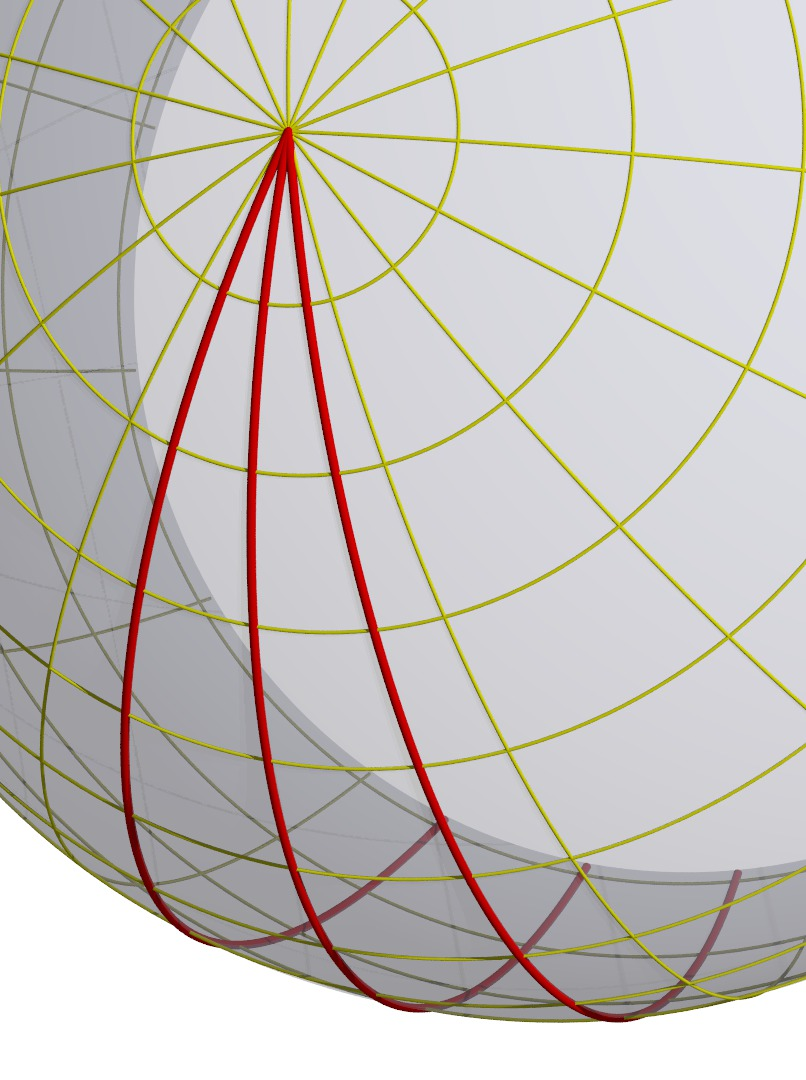
\includegraphics[height=6truecm]{chapters/3d/positiv.jpg}
\quad
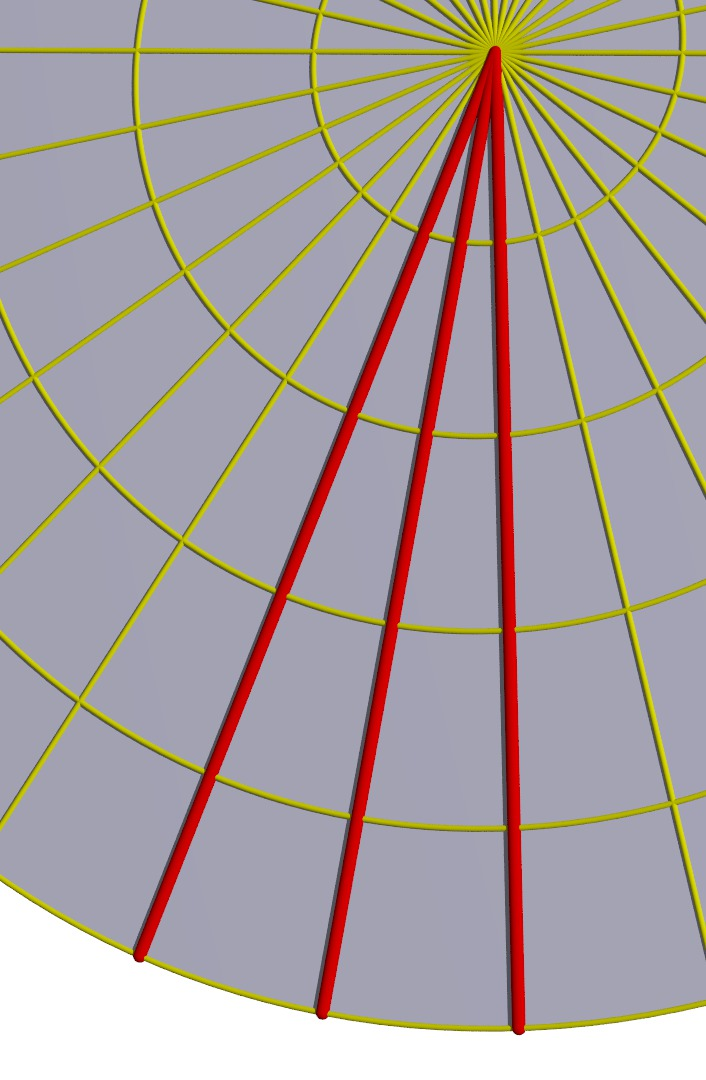
\includegraphics[height=6truecm]{chapters/3d/eben.jpg}
\quad
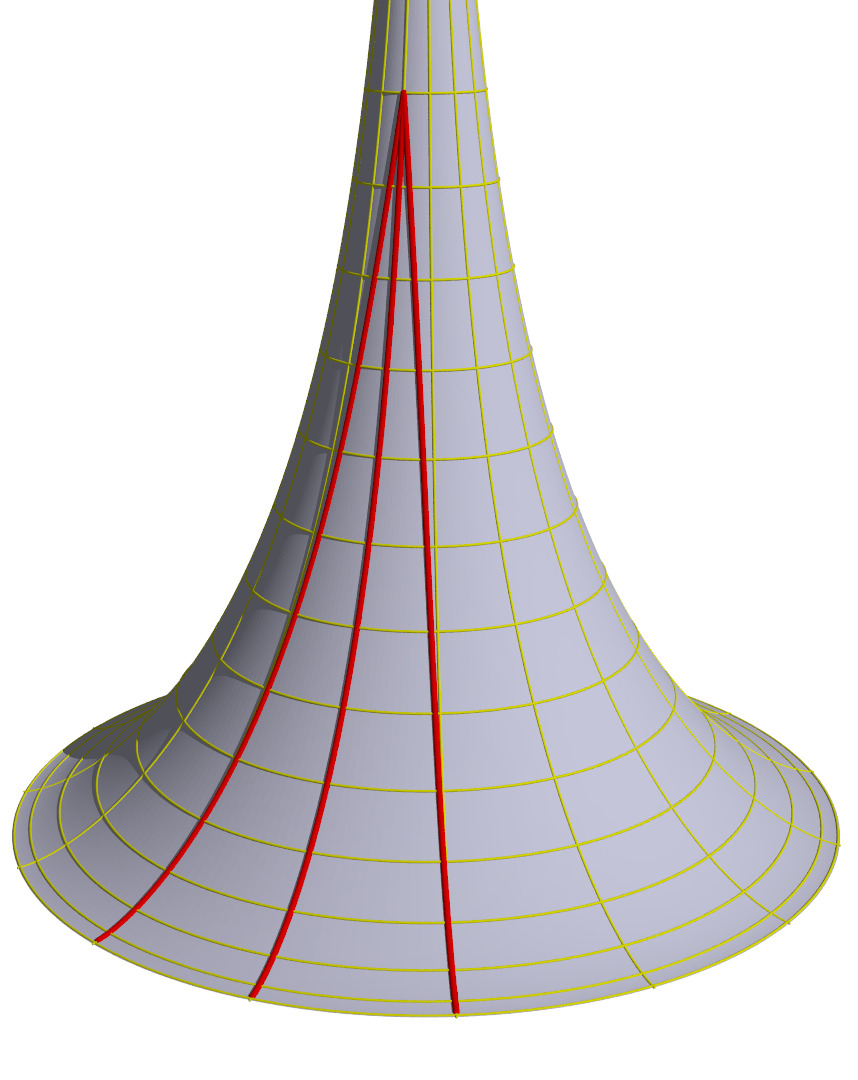
\includegraphics[height=6truecm]{chapters/3d/negativ.jpg}
\caption{Gleichschenklige Dreiecke mit gleichen Seitenlängen in einem
Universum mit positiver Krümmung (links), einem flachen Universum (Mitte)
und einem Universum mit negativer Krümmung (rechts).
Bei einem Universum mit positiver Krümmung ist der Winkel gegenüber
der kurzen Seite grösser als beim flachen Universum, bei einem
Universum mit negativer Krümmung ist er kleiner.
\label{skript:robertson:vergroesserung}}
\end{figure}
Ob das Universum positiv oder negativ gekrümmt oder gar flach ist,
muss experimentell bestimmt werden.
Dazu kann dazu den Winkel eines gleichschenkligen Dreiecks mit den
Seiten $l$ und $L$ mit $L\gg l$ verwenden.
In einem flachen Universum ist der Winkel gegenüber der Seite $l$
in Bogenmass $l/L$.
In einem Universum mit positiver Krümmung wird ein grösserer Winkel
beobachtet, in einem Universum mit negativer Krümmung ist der Winkel
dagegen kleiner.
Die Abbildung~\ref{skript:robertson:vergroesserung} veranschaulicht
diese vergrossernde Wirkung eines positiv gekrümmten Universums
und die verkleinernde Wirkung eines negativ gekrümmten Universums.

Um zu entscheiden, welchen Wert $\kappa$ für unser Universum hat,
kann man ein Dreieck verwenden, welches als $L$ die Entfernung zum kosmischen
Mikrowellenhintergrund verwendet.
Als kurze Seite des Dreiecks muss eine bekannte Grösse auf der
Fläche der letzten Streuung verwendet werden.
Zur Verfügung stehen Fluktuationen im kosmischen Mikrowellenhintergrund.
Man muss also die Entstehung und vor allem die Abmessungen solcher
Fluktuationen verstehen und berechnen können, bevor man den Test
durchführen kann.

\section{Steady State Universum}
\rhead{Steady State Universum}
Die Schlussfolgerung, dass das Universum vor relativ kurzer Zeit
aus einem heissen, dichten 
Zustand hervorgegangen sein müsse, war nicht von Anfang an akzeptiert.
Als alternative Hypothese wurde vorgeschlagen, dass im Universum 
zwar expandiert, dies aber schon seit ewigen Zeiten tut, und dass die
enstehenden
Lücken zwischen den Galaxien dadurch gefüllt werden, dass ständig
neue Materie entstand.
Dazu müsste pro Kubikkilometer und Jahr ein neues Wasserstoffatom
entstehen.

Diese Steady-State genannte Hypothese widerspricht jedoch zwei
im Folgenden diskutierten Beobachtungen.

\subsection{Olbers Paradoxon}
Wenn das Universum unendlich alt und gross ist, dann wird man in jeder
beliebigen Richtung nicht beliebig weit sehen können, sondern wird
irgendwann auf einen Stern treffen.
Der ganze Himmel müsste daher die Helligkeit von Sternen haben.

Nimmt man dagegen an, dass das Universum relativ jung ist, dann kann
man wegen der Endlichkeit der Lichtgeschwindigkeit nur soweit sehen,
wie das Alter des Universums erlaubt.

\subsection{Der kosmische Mikrowellenhintergrund}





